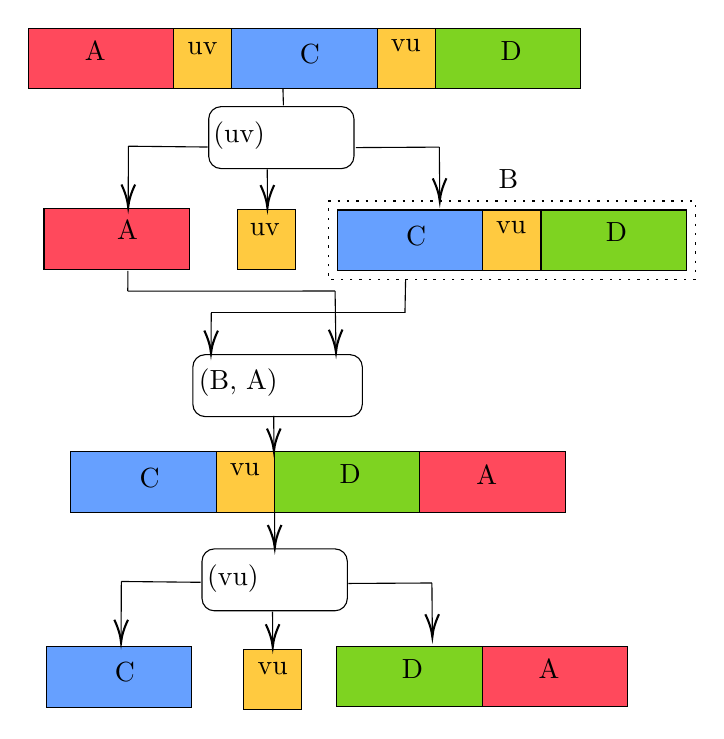
\begin{tikzpicture}[x=0.75pt,y=0.75pt,yscale=-1,xscale=1]
%uncomment if require: \path (0,390); %set diagram left start at 0, and has height of 390

%Shape: Rectangle [id:dp9893649794249966] 
\draw  [fill={rgb, 255:red, 255; green, 73; blue, 92 }  ,fill opacity=1 ] (52.05,3.05) -- (122.05,3.05) -- (122.05,32.19) -- (52.05,32.19) -- cycle ;
%Shape: Rectangle [id:dp8431641206368838] 
\draw  [fill={rgb, 255:red, 255; green, 202; blue, 64 }  ,fill opacity=1 ] (122.05,3.05) -- (150.19,3.05) -- (150.19,32.19) -- (122.05,32.19) -- cycle ;
%Shape: Rectangle [id:dp9464564998198169] 
\draw  [fill={rgb, 255:red, 102; green, 160; blue, 255 }  ,fill opacity=1 ] (150.19,3.05) -- (220.19,3.05) -- (220.19,32.19) -- (150.19,32.19) -- cycle ;
%Shape: Rectangle [id:dp4644107414908101] 
\draw  [fill={rgb, 255:red, 255; green, 202; blue, 64 }  ,fill opacity=1 ] (220.19,3.05) -- (248.33,3.05) -- (248.33,32.19) -- (220.19,32.19) -- cycle ;
%Shape: Rectangle [id:dp01734720754860286] 
\draw  [fill={rgb, 255:red, 126; green, 211; blue, 33 }  ,fill opacity=1 ] (248.33,3.05) -- (318.33,3.05) -- (318.33,32.19) -- (248.33,32.19) -- cycle ;
%Rounded Rect [id:dp44884729664756895] 
\draw   (139,46.8) .. controls (139,43.5) and (141.67,40.83) .. (144.97,40.83) -- (203.03,40.83) .. controls (206.33,40.83) and (209,43.5) .. (209,46.8) -- (209,64.7) .. controls (209,68) and (206.33,70.67) .. (203.03,70.67) -- (144.97,70.67) .. controls (141.67,70.67) and (139,68) .. (139,64.7) -- cycle ;
%Shape: Rectangle [id:dp12885984294517272] 
\draw  [fill={rgb, 255:red, 255; green, 73; blue, 92 }  ,fill opacity=1 ] (59.67,90.1) -- (129.67,90.1) -- (129.67,119.24) -- (59.67,119.24) -- cycle ;
%Shape: Rectangle [id:dp3326785133802803] 
\draw  [fill={rgb, 255:red, 255; green, 202; blue, 64 }  ,fill opacity=1 ] (152.71,90.25) -- (180.86,90.25) -- (180.86,119.4) -- (152.71,119.4) -- cycle ;
%Shape: Rectangle [id:dp22501821307072167] 
\draw  [fill={rgb, 255:red, 102; green, 160; blue, 255 }  ,fill opacity=1 ] (200.95,90.62) -- (270.95,90.62) -- (270.95,119.76) -- (200.95,119.76) -- cycle ;
%Shape: Rectangle [id:dp7752719637373938] 
\draw  [fill={rgb, 255:red, 255; green, 202; blue, 64 }  ,fill opacity=1 ] (270.95,90.62) -- (299.1,90.62) -- (299.1,119.76) -- (270.95,119.76) -- cycle ;
%Shape: Rectangle [id:dp8507110932325185] 
\draw  [fill={rgb, 255:red, 126; green, 211; blue, 33 }  ,fill opacity=1 ] (299.1,90.62) -- (369.1,90.62) -- (369.1,119.76) -- (299.1,119.76) -- cycle ;
%Shape: Rectangle [id:dp5311072976156744] 
\draw  [dash pattern={on 0.84pt off 2.51pt}] (196.69,86.27) -- (373.36,86.27) -- (373.36,124.11) -- (196.69,124.11) -- cycle ;
%Rounded Rect [id:dp3301360628536183] 
\draw   (131.36,166.29) .. controls (131.36,162.99) and (134.03,160.32) .. (137.32,160.32) -- (207.06,160.32) .. controls (210.35,160.32) and (213.02,162.99) .. (213.02,166.29) -- (213.02,184.19) .. controls (213.02,187.48) and (210.35,190.16) .. (207.06,190.16) -- (137.32,190.16) .. controls (134.03,190.16) and (131.36,187.48) .. (131.36,184.19) -- cycle ;
%Straight Lines [id:da9407555404294566] 
\draw [color={rgb, 255:red, 0; green, 0; blue, 0 }  ,draw opacity=1 ]   (199.89,129.67) -- (200.3,157.22) ;
\draw [shift={(200.33,159.22)}, rotate = 269.14] [color={rgb, 255:red, 0; green, 0; blue, 0 }  ,draw opacity=1 ][line width=0.75]    (10.93,-3.29) .. controls (6.95,-1.4) and (3.31,-0.3) .. (0,0) .. controls (3.31,0.3) and (6.95,1.4) .. (10.93,3.29)   ;
%Straight Lines [id:da10690320761239847] 
\draw [color={rgb, 255:red, 0; green, 0; blue, 0 }  ,draw opacity=1 ]   (100.02,129.72) -- (199.89,129.67) ;
%Straight Lines [id:da2639394928870016] 
\draw [color={rgb, 255:red, 0; green, 0; blue, 0 }  ,draw opacity=1 ]   (100.05,119.92) -- (100.02,129.72) ;
%Straight Lines [id:da27387399264242873] 
\draw [color={rgb, 255:red, 0; green, 0; blue, 0 }  ,draw opacity=1 ]   (140.23,140.14) -- (140.12,157.67) ;
\draw [shift={(140.11,159.67)}, rotate = 270.35] [color={rgb, 255:red, 0; green, 0; blue, 0 }  ,draw opacity=1 ][line width=0.75]    (10.93,-3.29) .. controls (6.95,-1.4) and (3.31,-0.3) .. (0,0) .. controls (3.31,0.3) and (6.95,1.4) .. (10.93,3.29)   ;
%Straight Lines [id:da07585390195908526] 
\draw [color={rgb, 255:red, 0; green, 0; blue, 0 }  ,draw opacity=1 ]   (140.23,140.14) -- (233.56,140.14) ;
%Straight Lines [id:da49250052279351275] 
\draw [color={rgb, 255:red, 0; green, 0; blue, 0 }  ,draw opacity=1 ]   (233.87,123.92) -- (233.56,140.14) ;
%Shape: Rectangle [id:dp018177126279713574] 
\draw  [fill={rgb, 255:red, 102; green, 160; blue, 255 }  ,fill opacity=1 ] (72.6,207.11) -- (142.6,207.11) -- (142.6,236.26) -- (72.6,236.26) -- cycle ;
%Shape: Rectangle [id:dp5026810470012354] 
\draw  [fill={rgb, 255:red, 255; green, 202; blue, 64 }  ,fill opacity=1 ] (142.6,207.11) -- (170.74,207.11) -- (170.74,236.26) -- (142.6,236.26) -- cycle ;
%Shape: Rectangle [id:dp6932736727959815] 
\draw  [fill={rgb, 255:red, 126; green, 211; blue, 33 }  ,fill opacity=1 ] (170.74,207.11) -- (240.74,207.11) -- (240.74,236.26) -- (170.74,236.26) -- cycle ;
%Shape: Rectangle [id:dp5569694264037944] 
\draw  [fill={rgb, 255:red, 255; green, 73; blue, 92 }  ,fill opacity=1 ] (240.71,207.11) -- (310.71,207.11) -- (310.71,236.26) -- (240.71,236.26) -- cycle ;
%Shape: Rectangle [id:dp4669156001238737] 
\draw  [fill={rgb, 255:red, 102; green, 160; blue, 255 }  ,fill opacity=1 ] (60.73,300.98) -- (130.73,300.98) -- (130.73,330.12) -- (60.73,330.12) -- cycle ;
%Shape: Rectangle [id:dp4276899357605074] 
\draw  [fill={rgb, 255:red, 126; green, 211; blue, 33 }  ,fill opacity=1 ] (200.76,300.87) -- (270.76,300.87) -- (270.76,330.01) -- (200.76,330.01) -- cycle ;
%Shape: Rectangle [id:dp5258868534842586] 
\draw  [fill={rgb, 255:red, 255; green, 73; blue, 92 }  ,fill opacity=1 ] (270.74,300.87) -- (340.74,300.87) -- (340.74,330.01) -- (270.74,330.01) -- cycle ;
%Rounded Rect [id:dp12564912499294212] 
\draw   (135.78,259.87) .. controls (135.78,256.57) and (138.45,253.9) .. (141.74,253.9) -- (199.81,253.9) .. controls (203.11,253.9) and (205.78,256.57) .. (205.78,259.87) -- (205.78,277.77) .. controls (205.78,281.06) and (203.11,283.73) .. (199.81,283.73) -- (141.74,283.73) .. controls (138.45,283.73) and (135.78,281.06) .. (135.78,277.77) -- cycle ;
%Shape: Rectangle [id:dp08095777599212983] 
\draw  [fill={rgb, 255:red, 255; green, 202; blue, 64 }  ,fill opacity=1 ] (155.76,302.31) -- (183.9,302.31) -- (183.9,331.46) -- (155.76,331.46) -- cycle ;
%Straight Lines [id:da21657498248500584] 
\draw [color={rgb, 255:red, 0; green, 0; blue, 0 }  ,draw opacity=1 ]   (174.78,32.44) -- (175,40.17) ;
%Straight Lines [id:da582963559957743] 
\draw [color={rgb, 255:red, 0; green, 0; blue, 0 }  ,draw opacity=1 ]   (100.33,59.89) -- (100.21,87.29) ;
\draw [shift={(100.21,89.29)}, rotate = 270.25] [color={rgb, 255:red, 0; green, 0; blue, 0 }  ,draw opacity=1 ][line width=0.75]    (10.93,-3.29) .. controls (6.95,-1.4) and (3.31,-0.3) .. (0,0) .. controls (3.31,0.3) and (6.95,1.4) .. (10.93,3.29)   ;
%Straight Lines [id:da990935754325963] 
\draw [color={rgb, 255:red, 0; green, 0; blue, 0 }  ,draw opacity=1 ]   (100.33,59.89) -- (138.49,60.29) ;
%Straight Lines [id:da9864693582766142] 
\draw [color={rgb, 255:red, 0; green, 0; blue, 0 }  ,draw opacity=1 ]   (167.22,71) -- (167.28,87.57) ;
\draw [shift={(167.29,89.57)}, rotate = 269.8] [color={rgb, 255:red, 0; green, 0; blue, 0 }  ,draw opacity=1 ][line width=0.75]    (10.93,-3.29) .. controls (6.95,-1.4) and (3.31,-0.3) .. (0,0) .. controls (3.31,0.3) and (6.95,1.4) .. (10.93,3.29)   ;
%Straight Lines [id:da5073093545210998] 
\draw [color={rgb, 255:red, 0; green, 0; blue, 0 }  ,draw opacity=1 ]   (250.11,60.33) -- (250.32,84.33) ;
\draw [shift={(250.33,86.33)}, rotate = 269.51] [color={rgb, 255:red, 0; green, 0; blue, 0 }  ,draw opacity=1 ][line width=0.75]    (10.93,-3.29) .. controls (6.95,-1.4) and (3.31,-0.3) .. (0,0) .. controls (3.31,0.3) and (6.95,1.4) .. (10.93,3.29)   ;
%Straight Lines [id:da2887459493739979] 
\draw [color={rgb, 255:red, 0; green, 0; blue, 0 }  ,draw opacity=1 ]   (209.89,60.56) -- (250.11,60.33) ;
%Straight Lines [id:da8299093498345442] 
\draw [color={rgb, 255:red, 0; green, 0; blue, 0 }  ,draw opacity=1 ]   (170.33,189.79) -- (170.42,204.87) ;
\draw [shift={(170.43,206.87)}, rotate = 269.66] [color={rgb, 255:red, 0; green, 0; blue, 0 }  ,draw opacity=1 ][line width=0.75]    (10.93,-3.29) .. controls (6.95,-1.4) and (3.31,-0.3) .. (0,0) .. controls (3.31,0.3) and (6.95,1.4) .. (10.93,3.29)   ;
%Straight Lines [id:da13698909135397708] 
\draw [color={rgb, 255:red, 0; green, 0; blue, 0 }  ,draw opacity=1 ]   (170.74,236.26) -- (170.83,251.34) ;
\draw [shift={(170.84,253.34)}, rotate = 269.66] [color={rgb, 255:red, 0; green, 0; blue, 0 }  ,draw opacity=1 ][line width=0.75]    (10.93,-3.29) .. controls (6.95,-1.4) and (3.31,-0.3) .. (0,0) .. controls (3.31,0.3) and (6.95,1.4) .. (10.93,3.29)   ;
%Straight Lines [id:da03134678203219754] 
\draw [color={rgb, 255:red, 0; green, 0; blue, 0 }  ,draw opacity=1 ]   (169.75,284.08) -- (169.84,299.16) ;
\draw [shift={(169.86,301.16)}, rotate = 269.66] [color={rgb, 255:red, 0; green, 0; blue, 0 }  ,draw opacity=1 ][line width=0.75]    (10.93,-3.29) .. controls (6.95,-1.4) and (3.31,-0.3) .. (0,0) .. controls (3.31,0.3) and (6.95,1.4) .. (10.93,3.29)   ;
%Straight Lines [id:da9696938749952316] 
\draw [color={rgb, 255:red, 0; green, 0; blue, 0 }  ,draw opacity=1 ]   (96.9,269.6) -- (96.79,297) ;
\draw [shift={(96.78,299)}, rotate = 270.25] [color={rgb, 255:red, 0; green, 0; blue, 0 }  ,draw opacity=1 ][line width=0.75]    (10.93,-3.29) .. controls (6.95,-1.4) and (3.31,-0.3) .. (0,0) .. controls (3.31,0.3) and (6.95,1.4) .. (10.93,3.29)   ;
%Straight Lines [id:da8437875902340053] 
\draw [color={rgb, 255:red, 0; green, 0; blue, 0 }  ,draw opacity=1 ]   (96.9,269.6) -- (135.06,270) ;
%Straight Lines [id:da29160181773165217] 
\draw [color={rgb, 255:red, 0; green, 0; blue, 0 }  ,draw opacity=1 ]   (246.54,270.33) -- (246.74,294.33) ;
\draw [shift={(246.76,296.33)}, rotate = 269.51] [color={rgb, 255:red, 0; green, 0; blue, 0 }  ,draw opacity=1 ][line width=0.75]    (10.93,-3.29) .. controls (6.95,-1.4) and (3.31,-0.3) .. (0,0) .. controls (3.31,0.3) and (6.95,1.4) .. (10.93,3.29)   ;
%Straight Lines [id:da7890705976162032] 
\draw [color={rgb, 255:red, 0; green, 0; blue, 0 }  ,draw opacity=1 ]   (206.32,270.56) -- (246.54,270.33) ;

% Text Node
\draw (78.05,8.33) node [anchor=north west][inner sep=0.75pt]   [align=left] {A};
% Text Node
\draw (127.48,8.62) node [anchor=north west][inner sep=0.75pt]   [align=left] {uv};
% Text Node
\draw (225.48,7.48) node [anchor=north west][inner sep=0.75pt]   [align=left] {vu};
% Text Node
\draw (140,47) node [anchor=north west][inner sep=0.75pt]   [align=left] {\treapSplit(uv)};
% Text Node
\draw (181.71,9.67) node [anchor=north west][inner sep=0.75pt]   [align=left] {C};
% Text Node
\draw (278.38,8) node [anchor=north west][inner sep=0.75pt]   [align=left] {D};
% Text Node
\draw (93.67,94.52) node [anchor=north west][inner sep=0.75pt]   [align=left] {A};
% Text Node
\draw (157.57,95.83) node [anchor=north west][inner sep=0.75pt]   [align=left] {uv};
% Text Node
\draw (276.24,95.05) node [anchor=north west][inner sep=0.75pt]   [align=left] {vu};
% Text Node
\draw (232.81,97.24) node [anchor=north west][inner sep=0.75pt]   [align=left] {C};
% Text Node
\draw (329.14,95.57) node [anchor=north west][inner sep=0.75pt]   [align=left] {D};
% Text Node
\draw (277.48,69.9) node [anchor=north west][inner sep=0.75pt]   [align=left] {B};
% Text Node
\draw (133.02,165.91) node [anchor=north west][inner sep=0.75pt]   [align=left] {\treapJoin(B, A)};
% Text Node
\draw (147.88,211.54) node [anchor=north west][inner sep=0.75pt]   [align=left] {vu};
% Text Node
\draw (104.45,213.73) node [anchor=north west][inner sep=0.75pt]   [align=left] {C};
% Text Node
\draw (200.79,212.07) node [anchor=north west][inner sep=0.75pt]   [align=left] {D};
% Text Node
\draw (266.71,212.4) node [anchor=north west][inner sep=0.75pt]   [align=left] {A};
% Text Node
\draw (92.59,307.6) node [anchor=north west][inner sep=0.75pt]   [align=left] {C};
% Text Node
\draw (230.81,305.82) node [anchor=north west][inner sep=0.75pt]   [align=left] {D};
% Text Node
\draw (296.74,306.16) node [anchor=north west][inner sep=0.75pt]   [align=left] {A};
% Text Node
\draw (137,260.07) node [anchor=north west][inner sep=0.75pt]   [align=left] {\treapSplit(vu)};
% Text Node
\draw (161.33,307.31) node [anchor=north west][inner sep=0.75pt]   [align=left] {vu};


\end{tikzpicture}

